\begin{exercises} 
\item Let $f$ and $g$ be differentiable functions for which the following information is known:  $f(2) = 5$, $g(2) = -3$, $f'(2) = -1/2$, $g'(2) = 2$.
\ba
	\item Let $h$ be the new function defined by the rule $h(x) = g(x) \cdot f(x)$.  Determine $h(2)$ and $h'(2)$.
	\item Find an equation for the tangent line to $y = h(x)$ at the point $(2,h(2))$ (where $h$ is the function defined in (a)).
	\item Let $r$ be the function defined by the rule $r(x) = \frac{g(x)}{f(x)}$.  Is $r$ increasing, decreasing, or neither at $a = 2$?  Why?
	\item Estimate the value of $r(2.06)$ (where $r$ is the function defined in (c)) by using the local linearization of $r$ at the point $(2,r(2))$.
\ea
\begin{exerciseSolution}
\end{exerciseSolution}
\item Consider the functions $r(t) = t^t$ and $s(t) = \arccos(t)$, for which you are given the facts that $r'(t) = t^t(\ln(t) + 1)$ and $s'(t) = -\frac{1}{\sqrt{1-t^2}}$.  Do not be concerned with where these derivative formulas come from.  We restrict our interest in both functions to the domain $0 < t < 1$.
\ba
	\item Let $w(t) = t^t \arccos(t)$.  Determine $w'(t)$.
	\item Find an equation for the tangent line to $y = w(t)$ at the point $(\frac{1}{2}, w(\frac{1}{2}))$.
	\item Let $v(t) = \frac{t^t}{\arccos(t)}$.  Is $v$ increasing or decreasing at the instant $t = \frac{1}{2}$?  Why?
\ea
\item Let functions $p$ and $q$ be the piecewise linear functions given by their respective graphs in Figure~\ref{F:2.3.Ez3}.  Use the graphs to answer the following questions.
\begin{figure}[h]
\begin{center}
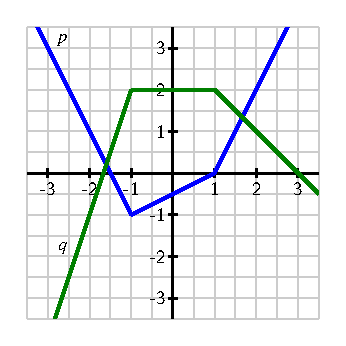
\includegraphics{figures/2_1_Ez3.eps}
\caption{The graphs of $p$ (in blue) and $q$ (in green).} \label{F:2.3.Ez3}
\end{center}
\end{figure}
\ba
	\item Let $r(x) = p(x) \cdot q(x)$.  Determine $r'(-2)$ and $r'(0)$.
	\item Are there values of $x$ for which $r'(x)$ does not exist?  If so, which values, and why?
	\item Find an equation for the tangent line to $y = r(x)$ at the point $(2,r(2))$.
	\item Let $z(x) = \frac{q(x)}{p(x)}$.  Determine $z'(0)$ and $z'(2)$.
	\item Are there values of $x$ for which $z'(x)$ does not exist?  If so, which values, and why?	
\ea
\item A farmer with large land holdings has historically grown a wide variety of crops.  With the price of ethanol fuel rising, he decides that it would be prudent to devote more and more of his acreage to producing corn.  As he grows more and more corn, he learns efficiencies that increase his yield per acre.  In the present year, he used 7000 acres of his land to grow corn, and that land had an average yield of 170 bushels per acre.  At the current time, he plans to increase his number of acres devoted to growing corn at a rate of 600 acres/year, and he expects that right now his average yield is increasing at a rate of 8 bushels per acre per year.  Use this information to answer the following questions.
\ba
	\item Say that the present year is $t = 0$, that $A(t)$ denotes the number of acres the farmer devotes to growing corn in year $t$, $Y(t)$ represents the average yield in year $t$ (measured in bushels per acre), and $C(t)$ is the total number of bushels of corn the farmer produces.  What is the formula for $C(t)$ in terms of $A(t)$ and $Y(t)$?  Why?
	\item What is the value of $C(0)$?  What does it measure?
	\item Write an expression for $C'(t)$ in terms of $A(t)$, $A'(t)$, $Y(t)$, and $Y'(t)$.  Explain your thinking.
	\item What is the value of $C'(0)$?  What does it measure?
	\item Based on the given information and your work above, estimate the value of $C(1)$.	
\ea
\item Let $f(v)$ be the gas consumption (in liters/km) of a car going at velocity $v$ (in km/hour). In other words, $f(v)$ tells you how many liters of gas the car uses to go one  kilometer if it is traveling at $v$ kilometers per hour. In addition, suppose that $f(80)=0.05$ and $f'(80) = 0.0004$.
\ba
	\item Let $g(v)$ be the distance the same car goes on one liter of gas at velocity $v$.  What is the relationship between $f(v)$ and $g(v)$? Hence find $g(80)$ and $g'(80)$.
      	\item Let $h(v)$ be the gas consumption in liters per hour of a car going at velocity $v$. In other words, $h(v)$ tells you how many liters of gas the car uses in one hour if it is going at velocity $v$.   What is the algebraic relationship between $h(v)$ and $f(v)$?  Hence find $h(80)$ and $h'(80)$.     
	\item How would you explain the practical meaning of these function and derivative values to a driver who knows no calculus?  Include units on each of the function and derivative values you discuss in your response.  
\ea
\end{exercises}
\afterexercises